\begin{figure}[htbp]
\centering
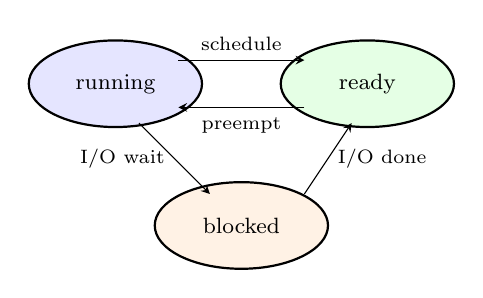
\begin{tikzpicture}[font=\footnotesize, >=stealth, x=1cm, y=1cm]
  \draw[thick,fill=blue!10] (0,2.6) ellipse (1.1 and 0.55);
  \node at (0,2.6) {running};
  \draw[thick,fill=green!10] (3.2,2.6) ellipse (1.1 and 0.55);
  \node at (3.2,2.6) {ready};
  \draw[thick,fill=orange!10] (1.6,0.8) ellipse (1.1 and 0.55);
  \node at (1.6,0.8) {blocked};
  \draw[->] (0.8,2.9) -- (2.4,2.9) node[midway,above]{\scriptsize schedule};
  \draw[->] (2.4,2.3) -- (0.8,2.3) node[midway,below]{\scriptsize preempt};
  \draw[->] (0.3,2.1) -- (1.2,1.2) node[midway,left]{\scriptsize I/O wait};
  \draw[->] (2.4,1.2) -- (3.0,2.1) node[midway,right]{\scriptsize I/O done};
\end{tikzpicture}
\caption{The three-state life of a process. The scheduler moves a
process between ready and running; the I/O system moves it between
running and blocked. Everything else --- priorities, queues,
timeslices --- is policy on top of this machine.}
\label{fig:states12}
\end{figure}
